\section{Model Development}

\subsection{Data Synchronisation and Post-Processing}
Before being able to use the data for training, we needed to synchronise the data recorded from the smartphone, and the fbx data from the MoCap studio.
To do this we derived the acceleration of the phone based on the MoCap data to find where it meets/exceeds the magnitude of the shake recorded by the app. From this we can determine the frame of the fbx data that corresponds to the recorded timestamp. We can determine the frame for any subsequent timestamp based on the known frame-rate of 60fps. 
To verify the data didn't drift we resync the data based on the other 2 recorded shakes, verifying that they're within 10 frames of the expected frame. In doing this verification, we did not come across any recording wherein subsequent shakes were not found to be at the expected frame.
The synchronisation was performed with a Python script that was run within Blender after loading in the fbx.
Blender was used as it permitted viewing the fbx data so that we could verify the frames the shake was detected by watching the playback. We could also use Blender to verify the derived location, roll, pitch, and yaw were correct by inserting a plane into the scene and assigning it the derived values, checking that it lined-up through all of the motion trackers.
The other reason for using Blender is that it allowed us to programmatically access the fbx file as a data structure and therefore write a script capable of deriving the required head and phone poses from the fbx, and then sync it with the data recorded from the phone.
Synchronised data was exported to CSVs for each motion recording, containing a path to the image, the raw IMU data, and the derived MoCap data.
\tempnote{Link to script used: \url{https://github.com/whattheforkbomb/dissertation_code/blob/trunk/datacollection/dataSynchronisation.py}}

An additional stage of pre-processing that was performed was to generate the RGB images from the YUV data captured by the phone. This was performed with a Python script and the OpenCV library.\tempnote{Link to script used.}
% script.processor.process_data('G:/Study/7', 1900)
% script.processor.process_data('G:/Study/6', 8900)
% script.processor.process_data('G:/Study/5', 9500)
% script.processor.process_data('G:/Study/4', 900)
% script.processor.process_data('G:/Study/3', 20000)
% script.processor.process_data('G:/Study/2', -320, attempt_0_override=-320)
% script.processor.process_data('G:/Study/1', 1000)
% script.processor.process_data('G:/Study/0', 3000)

\subsection{The Proposed Models} % TODO: Drop /s if only one model % The Proposed System
% Both models then used to train HMM, evaluate which performs better
% In this section we shall propose two models for quantising the motion of the phone and position of the head, and a HMM to classify sequences of the encoded motion as specific gestures.
In this section we shall propose a CNN for encoding the direction of linear and angular movement observed between 2 frames, and a RNN to classify sequences of encoded movement as a gesture.
% Possibly one-hot encoding

We opted to split the development of our model into to pieces for 
The purpose of splitting our proposed model into 2 distinct models (the CNN and RNN) is two-fold:

\nl\textbf{Obtaining the Face Pose}\nl
To be able to track the movement of the face, we first need to extract it and determine its pose.

\nl\textbf{Reduce the Observation Space For the RNN}\\
Since the acceleration can be any value, and the position of the face in the image also any range of values, to use them as raw inputs to a HMM would require a significant amount of data to ensure we have samples that cover the training space.
By first encoding the data we can reduce the possible training space.
The simplest way to perform this would be to quantise the data. This would involve reducing the resolution of the data, for example mapping all the angles of rotation into a smaller range, as was performed by \citeauthor{elmezain2008hidden} to convert the movement of a hand capture in a sequence of images to the angle of the movement~\cite{elmezain2008hidden}, reducing the possible input to their HMM to just 19 observable states.

\subsubsection{Movement Encoding}\nl
% Want to reduce the possible observation states we need to learn for our classification HMM.
% \nl\textbfit{Classifier 1}\nl
% 2: Cascading motion encoder
%   No transfer learning
%   use YuNet to preprocess the image. 
%   - If no face found then return no encoding for face
%   - Else feed into NN to encode the motion
%   Acceleration encoded manually, just quantise and see if over given amount, then convert to encoding
For this model we take inspiration from the cascading classifiers we reviewed~\cite{kim2017real, neto2012real, francone2011using,viola2004robust}, wherein we will utilise the YuNet face detection CNN~\cite{yu2022yunet} which is used with OpenCV to extract the bounding box of the face, and the positions of the eyes, nose, and mouth corners. To improve robustness of the classifier we will reduce the input image size down to 320x180, from the 1280*720 resolution we captured.

If no face is found we simply return a state representing no face detected, otherwise we will quantise the output by dividing the values by 10, and round to the nearest int. This will reduce the total possible values from 0-57,600 to 0-576.
Once the values have been quantised, they will be fed into a new model which we will train to predict the roll, pitch, and yaw of the face.
This is a small Fully Connected Network which will be trained on YuNet outputs, trying to predict a quantised roll, pitch, and yaw that we will generate from the MoCap data.
We do not need to try and predict the position of the head using the MoCap data as YuNet already gives use the position of the head in the frame. We will then return the quantised position of the face bounding box and landmarks, along with the quantised pose of the head predicted by by our model.
Acceleration will be quantised in the same manner, multiplying by 5 and rounding to the nearest int. This should remove some noise and minor adjustments to the phone's position, and only track movements over 0.2ms\textsuperscript{-2}.

To build this model we will be using TensorFlow, with the Keras API, as TensorFlow provides as Mobile version of the network that can be run on smartphones.

\begin{figure*}
    \centering
    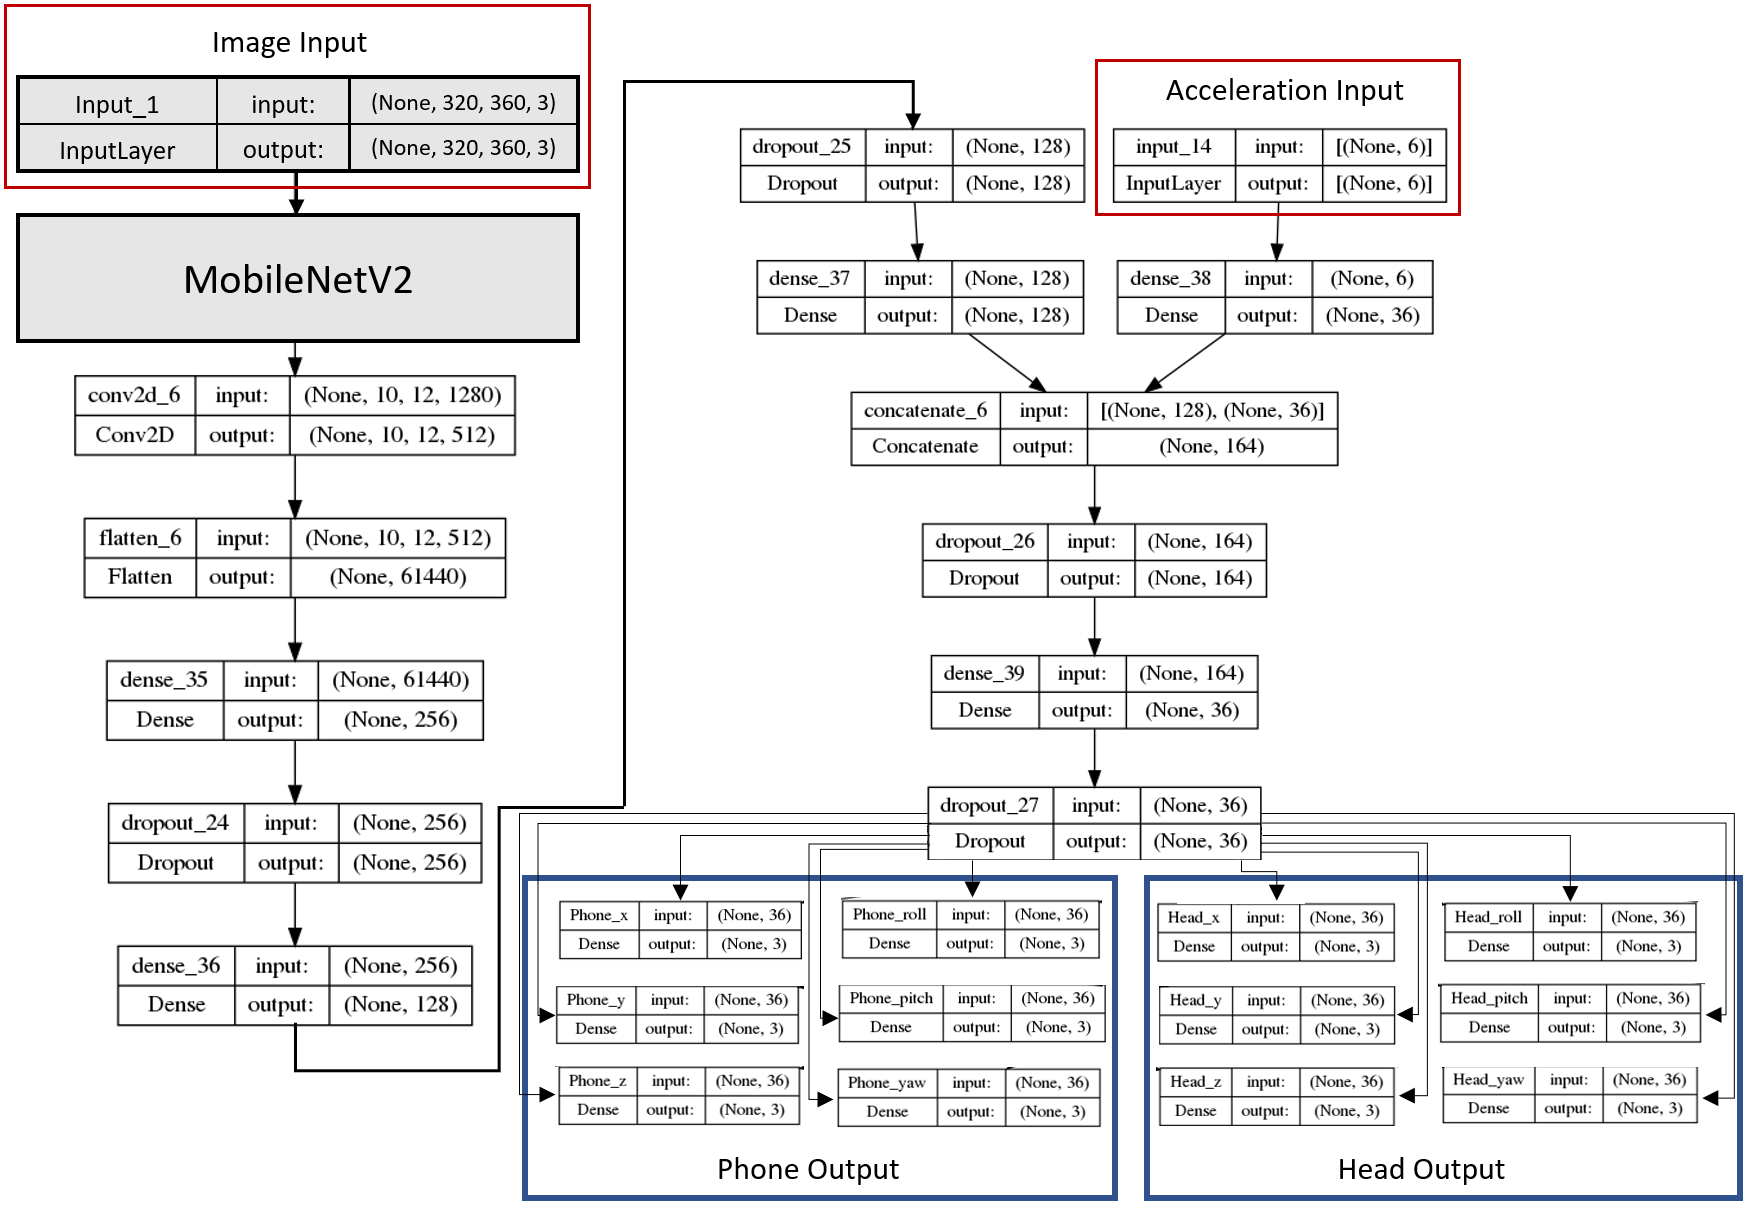
\includegraphics[width=0.9\textwidth]{figures/TL_Model_Clean.png}
    \caption{\label{fig:motion_encoder} Motion Encoder Model}
    \Description{Diagram of the motion encoder model, showing the image inputs feeding into the MobileNetV2 model, the acceleration input being joined with the output of the mobile net and subsequent dense layers, and the 12 expected output.}
\end{figure*}

% might encode one-hot instead, in which case take two sequential inputs and calculate the movement

% \nl\textbfit{Classifier 2}\nl
% % 2: NN using transfer learning (using image net model, which one?).
% %   Use tensorflow (work with current cuda and dependencies?) or pytorch?
% %   - 4 inputs, 2 images, 2 sets of acceleration data
% %     Images fed into own image net model, outputs into FCN and then both connected into FCN
% %     Acceleration fed into FCN, then joined with FCN of images
% %   Output one-hot encoded direction of motion for each DoF
% %   might be slow as re-processing previous image
% Our second proposed model we will be using transfer learning to extend an existing CNN trained on image net to predict the direction of motion, in each degree of freedom for both the head and phone, observed between two frames.
% We could try to emulate the YuNet model, and output the head pose and position, a lack of 
% One issue is lack of images not containing face, how to handle if no face detected?


\subsubsection{Gesture Classification}\nl
% Could have used an RNN bolted directly onto the back of the classifiers
Once we have our quantised observations from our cascade, we can now look to classifying the sequence of these observations as gestures.
For this we have chosen to train a HMM, as it will allows us to encode the gestures as the hidden state, with the quantised data as the observed states.

To build and train this we will first collect the output from out first model to generate the training data required. This will give us the data sequences we would expect to see in different gestures.
To build the HMM we will use the HMMLearn python package. Implementation of the model in this scenario shouldn't matter as much as our previous model as evaluating a HMM is much more trivial than a neural network. You should be able to export the state and variables of the HMM and transfer these to any other language or framework.
From here learning the hidden states is straight-forward, as we simply need to provide the 

% How account for different sample rates? How include this as part of observation state?

% If we have no transfer learning
% To achieve our goal we opted to build a model of 3 parts.
% \\\tempnote{Would be 2 parts if can get transfer learning to work, but having issues. Will just leave as preprocessing of the image prior to feeding into model if unable to get it sorted.}\\
% The first stage is to identify if a face is present in an image. For this we utilise a prebuilt CNN which returns a bounding box of the face, along with the points of the eyes, nose, and mouth corners~\cite{yu2022yunet}. %This is executed with OpenCV
% The bounding box and the landmarks, along with the average of the IMU data since the last image, are then passed into a neural network which aims to predict how the head and phone are moving through the 6 Degrees of freedom.
% If no bounding box or landmarks are found for a given image, we provide the previous bounding box and landmarks. Ideally we would not provide anything, however the network expects to 
% \tempnote{is input going to be padded with zeros for first frames / last frames, or require certain number of frames before attempting classification?}\\
% The second model is 2 models which will be trained to predict the direction of movement in each of the 6 DoF for the head and phone (the head model will also take the landmarks and bounding box as input).
% It will output as a 2d one-hot encoded array, each row being the Degree of Freedom, the column being the direction (0 = stationary, -1 = negative, +1 = positive).
% The output of the 2 can then be fed into a HMM trained to predict the gesture performed based on the derived motion. (possibly an RNN if easier)

% What models have been used for cascading (facial landmark and YuNet CNNs)

% Tools, issues

\subsubsection{Training}\nl
% Breakdown of samples (train, validation, test), and count
Prior to training the first half of proposed model, we wanted to increase the amount of effective data we have for training we performed some fps scaling of the data. 
This involved iterating through our collected data and only extracting frames if they \textit{would} have been available at a lower sample rate. For images and the MoCap data we simply took the last available data for the current timestamp, but for the accelerations we calculated the average based on the time elapsed, as using just the last value would not be representative of the acceleration of the phone during the period.
In deployment of the model this would require that the accelerations are averaged in between images being captured, but this should provide greater resolution on how the phone is moving.\\
\tempnote{link to repo with python notebook for doing the fps scaling, took 3hr, 40min to generate 1756361 input: 5fps - 7997, 10fps - 4971, 15fps - 4451, fps20 - 4184, Un-aggregated (\~32fps) - 1029, Number of files to process: 22632, Testing paths: 4527, Training: 12673, Validation: 5432}\\
\tempnote{script: \url{https://github.com/whattheforkbomb/dissertation_code/blob/trunk/dataprocessing/data_analysis.ipynb}, \url{https://github.com/whattheforkbomb/dissertation_code/blob/trunk/datacollection/imageGenerator.py}}
% Only 10 \& 15 fps files Number of files to process: 9422 - Testing paths: 1885, Training: 6029, Validation: 1508
% \tempnote{Additionally generated the required classification output for the motion encoders.}
% Only 10 fps files Number of files to process: 4971 Testing paths: 995, Training: 3180, Validation: 796

% 1028 recordings of gestures.
% K-Fold validation

% Hyper-params (quantisation, image size (if transfer learning?), fps scales)
% Image input sizes

\tempnote{Training notebook: \url{https://github.com/whattheforkbomb/dissertation_code/blob/trunk/training/training.ipynb}}


